% 118-99(118쪽) — 한 변의 길이가 6인 정사각형에서 각 변의 중점을 이어 만든 4개의 정사각형 중
% 오른쪽 위의 것을 색칠하는 시행을 되풀이한 그림(원문 「오른쪽 그림」). 스캔 화질이 낮아 TikZ 로 다시 그림.
% 원문처럼 3회 시행까지만 그리고(색칠 1 + 3 + 9개), 라벨은 원문에 있는 「6」 하나뿐이다.
% 20회 반복한 넓이의 합(답)이 그림에서 읽히지 않게 눈금·넓이 값은 적지 않는다.
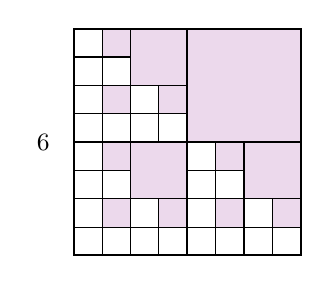
\begin{tikzpicture}[x=0.36cm, y=0.36cm, line width=0.5pt]
  % 1회 시행 — 오른쪽 위 정사각형
  \fill[violet!15] (4,4) rectangle (8,8);
  % 2회 시행 — 남은 3개의 정사각형에서 각각 오른쪽 위
  \foreach \a/\b in {0/4, 0/0, 4/0}{
    \fill[violet!15] (\a+2,\b+2) rectangle (\a+4,\b+4);
  }
  % 3회 시행 — 남은 9개의 정사각형에서 각각 오른쪽 위
  \foreach \a/\b in {0/4, 0/6, 2/4, 0/0, 0/2, 2/0, 4/0, 4/2, 6/0}{
    \fill[violet!15] (\a+1,\b+1) rectangle (\a+2,\b+2);
  }
  % 1회 시행의 중점을 이은 선
  \draw[line width=0.6pt] (4,0) -- (4,8);
  \draw[line width=0.6pt] (0,4) -- (8,4);
  % 2회 시행의 중점을 이은 선
  \foreach \a/\b in {0/4, 0/0, 4/0}{
    \draw (\a+2,\b) -- (\a+2,\b+4);
    \draw (\a,\b+2) -- (\a+4,\b+2);
  }
  % 3회 시행의 중점을 이은 선
  \foreach \a/\b in {0/4, 0/6, 2/4, 0/0, 0/2, 2/0, 4/0, 4/2, 6/0}{
    \draw[line width=0.4pt] (\a+1,\b) -- (\a+1,\b+2);
    \draw[line width=0.4pt] (\a,\b+1) -- (\a+2,\b+1);
  }
  \draw[line width=0.7pt] (0,0) rectangle (8,8);
  \node[anchor=east, font=\small] at (-0.5,4) {$6$};
\end{tikzpicture}
